\section{Local-file continuation and mechanism measurements}
This continuation supersedes the current scientific figures for 2--4, S1, S6--S8 and S10--S13. Previous data and plots remain in their labeled cohort directories. No earlier event identifier is silently reused in the new cohort. All new empirical points come from observed waveforms and this implementation's saved calculations; theoretical FK Green functions are predictions, not observations. Published images occur only in the separate comparison PDF.

\paragraph{Inputs and actual processing.}
Fourteen previously omitted files were processed: six original CAAM/COLB template windows, seven short local-archive records, and the original CSOB benchmark window. These event-selected observations do not measure continuous discovery exposure. Twenty previously unattempted public requests were issued: 19 returned readable files and one CPIS interval returned HTTP 204; zero failed and no previously attempted interval was retried. All 33 files entered PhaseNet. Compatible older per-file inference and day-association results were reused only after observation, model and settings checks. Raw observation hashes, short-window classifications and processing receipts are in \path{data/local_extension}.

The new checkpoint has 1,024 files, 30 station names, 87 channels and 8,952.452 union channel-hours, an increase of 245.482 hours. Four added names occur only in short single-channel records. Response epochs cover 8,952.386 hours; four short intervals totaling 0.0667 hours lack valid responses. Ten picks at CROS, V0102 and V0105 lack verified association metadata and remain in \path{picks_without_metadata.csv}. The independent selection contains 136,376 picks, 7,416 associated picks and 1,024 provisional events. Requests with no returned observations are not exposure. The frozen queue has 842 downloads, 36 empty responses, 11 failures and 73,917 pending requests. Full study-period coverage remains unfinished. The alternative Tramelli (2021) association profile is retained and explicitly prevents an exact starting-model claim.

\paragraph{Calibration and relocation outcomes.}
All nine requested calibration/downstream stages exited successfully; scientific acceptance is false. The new 921-event causal input supplies 38 numerical calibration candidates, 219 VELEST filter passes and 123 final relocated gap passes. Two fixed-grid TomoDD rounds, 80 conditional SVD estimates, 67 provisional amplitude magnitudes and 122 CPOZ component gathers were recomputed for this cohort. On 398 shared waveform differential observations, residual RMS decreases from 0.04125 to 0.03940 s; on 4,367 shared picked differences, from 0.10738 to 0.10130 s. The maximum between-round shift is 386 m horizontally and 0.372 km vertically. Thirty-four retained events have no cross-correlation link and none has more than 100. S9 therefore still has no qualifying result.

Full 32/64-bit calibration paths differ by 558 m horizontally, 0.89 km in depth, 0.32 km/s in velocity and 0.25 s in station delay. Identical converged starts give identical printed coordinates and velocities; this does not remove accumulated nonlinear sensitivity. Regional-start depth differences reach 1.04 km. Earlier instrumentation and failed held-out validation are retained as historical evidence, not asserted to have been rerun for this extension. The new association at 29 January 2022 06:26:03.080 UTC has one P and five S picks. Its reported VELEST RMS increases 0.44, 0.45, 0.46 s in the first three passes; residual rejection leaves too few picks, so it does not survive. The final 123 origins match the prior cohort, with coordinate differences at most 0.001 km vertically. More input did not yield another accepted or retained event.

The relocated-subset magnitude inversion uses 5,887 measured channels, 1,623 SNR passes and 884 relative-amplitude equations. Routine duration magnitude is a documented external calibration prior. Conditional $M_c=0.0$ and $b=0.866\pm0.110$ describe 41 selected magnitudes, not population completeness. There are 383 positive observed S--P pairs, with 0.1777 s RMS against the approximate own model; 42 deep events are flagged for review. These checks do not validate absolute depths.

\paragraph{Polarity and amplitude review.}
The frozen eight-event candidate set preserves the requested event 649 identifier. All 180 available station-event records were inspected visually by the AI; none was reviewed by a human seismologist. Responses verify the upward vertical orientation. First motions were read from counts and response-corrected velocity without an additional bandpass. Accepted and rejected judgments, trace references and reasons are saved in \path{data/mechanism_followup/review_decisions.csv}. Some initially assigned signs describe later lobes rather than first motions and were corrected. The 13 additional stations for 649 were inspected: CGAU, CLAC, CSOC, CBAG, CCAP, CFMN, CMSN, CMTS, COLB, CPIS, CQUE, CRUS and CUMA. The new AI-reviewed CFMN P arrival is 20 March 2025 06:32:18.910 UTC, with approximately 0.03 s reading uncertainty; it is not an author pick.

S/P is the ratio of peak three-component velocity norms in independently aligned P and S windows, filtered 1--15 Hz. P uses P to min(P+0.30,S-0.10) s, S uses S to S+0.50 s; noise uses P-3 to P-1 s. Both peak/noise-RMS ratios must exceed three. Of 61 automated measurement passes, 41 retain visually usable phase packets; 29 first motions survive AI review. These explicit exploratory windows are not asserted to recover Tan's unpublished per-event choices. Seven events have fewer than eight reliable polarities. Event 649 has eight, but SKHASH's computed azimuthal gap is 96.57 degrees, above the unchanged 90-degree limit. The successful software run returns zero solutions, not a negative finding about faulting style.

\paragraph{FK and gCAP trials.}
Official generic FK 3.3 and Zhu's generic gCAP source were inspected and compiled; archive examples, example results and plotting scripts were excluded. Source URLs, archive hashes and extracted member lists are in \path{data/mechanism_followup/method_resources.json}. The gCAP distribution requires unavailable Numerical Recipes and SAC filtering functions. A separately named port replaces its three-dimensional curvature eigensolver with a Jacobi calculation and filters complete observations/Green functions externally before fitting. The fixed-matrix eigensolver check differs from NumPy by at most $6.7\times10^{-8}$; this is a software test, not an empirical result. External filtering differs from stock segment filtering and limits exact reproduction.

Seven candidates supply at least four reviewed three-component stations; 698 supplies only one. FK generates nine double-couple components per station using the independently fitted four-layer provisional model. Depth is below sea level, with the model surface at $-0.5$ km; source depth is shifted by +0.5 km. Individual receiver topography is not corrected. Density uses the documented FK fallback $\rho=0.77+0.32V_p$ in g/cm$^3$; $Q_S=500$, $Q_P=1000$ are defaults, not measured properties. Verified components rotate to up, outward radial and counterclockwise transverse in cm/s. Horizontal-energy consistency passes.

Both frequency trials use fixed own locations/depths, a 10-degree double-couple grid, 0.1 magnitude increments and a 0.2 s source duration. Pnl windows are P-0.3 to P+1.2 s; surface-wave windows S-0.3 to S+4.7 s, with maximum shifts 0.5 and 1 s, Pnl weight two and distance exponents one and one-half. These are disclosed assumptions. The two bands are 0.2--2 and 1--5 Hz. All seven fits return finite numerical outputs, but variance reduction remains poor and orientations are strongly frequency-dependent. No solution is accepted; no SKHASH--gCAP comparison can be computed without a SKHASH solution. The rotation below compares two own gCAP trials only.

\begin{center}\small\begin{tabular}{rrrrrr}\toprule Event & P signs & S/P & VR low (\%) & VR high (\%) & Rotation ($^\circ$)\\\midrule
212 & 3 & 5 & 6.9 & 7.1 & 79.0\\
312 & 5 & 5 & 11.9 & 7.0 & 73.7\\
315 & 4 & 4 & 14.8 & 6.4 & 97.9\\
359 & 3 & 7 & 7.3 & 3.9 & 48.3\\
373 & 2 & 4 & 3.9 & 5.0 & 34.2\\
649 & 8 & 10 & 6.0 & 4.2 & 79.1\\
698 & 1 & 1 & --- & --- & ---\\
815 & 3 & 5 & 9.2 & 2.3 & 80.6\\
\bottomrule\end{tabular}\end{center}
Event-specific requirements, logs, controls, observed SAC inputs, theoretical Green functions and fitted traces are retained under \path{data/mechanism_followup}. For 649, another reliable first motion in the uncovered sector or justified review of current ambiguous onsets is required even to pass the SKHASH gap gate. Additional stations are not automatically usable polarities. For every other candidate the insufficient polarity count is recorded explicitly. Accepted waveform mechanisms further require defensible source locations/model, reviewed windows and stable fits; an optimizer returning angles does not establish these conditions.

\begin{figure}[H]\centering
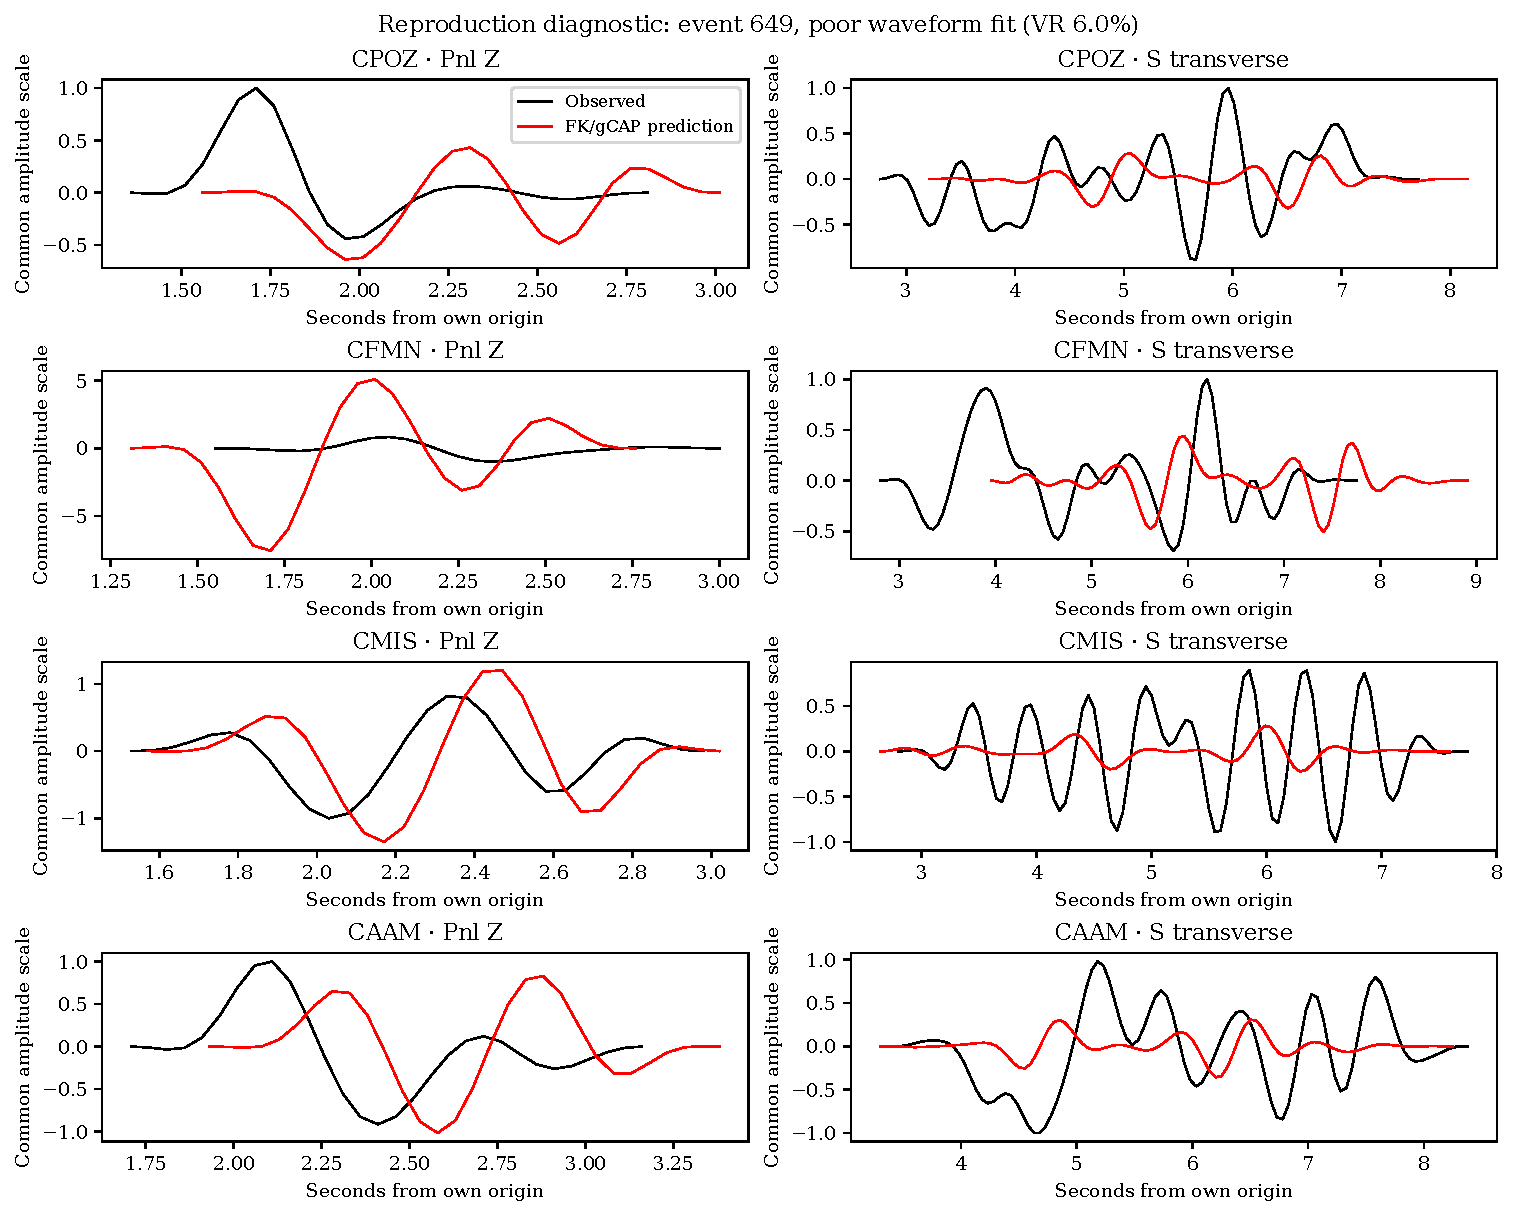
\includegraphics[width=.97\linewidth]{figures/mechanism_fit_diagnostic.pdf}
\caption{Reproduction diagnostic, not a publication figure: event 649 observations and FK/gCAP predictions at four stations. Each pair shares the observed-peak amplitude normalization; the prediction is not normalized separately. Pnl and transverse-S discrepancies explain why the trial beachball is unaccepted.}
\end{figure}

\paragraph{Rebuild, provenance and replacements.}
Run \path{.venv/bin/python scripts/rebuild_local_followup.py} to validate saved manifests, redraw these panels, integrate their records and compile both documents. The option \path{--analysis} reruns the frozen inference/association, calibration/downstream stages and mechanism calculations from retained observations; it does not download a new waveform batch or replace AI review with an automatic claim of human review. Successful commands from this continuation are recorded in \path{data/local_extension/execution.json} and mechanism execution logs; old inference caches were hash-checked, not recomputed from scratch. The original waveform inputs remain local with source receipts and hashes. The source and result files superseded in the current documents are listed in \path{docs/local_followup.md}; historical numerical cohorts remain unchanged.
